\section{Fase di implementazione}
\subsection{Linguaggi}
\subsubsection{HTML}
Il linguaggio di markup scelto per realizzare tutte le pagine del sito è XHTML. Si è preferito questo a HTML5 per i seguenti motivi:
\begin{itemize}
    \item garantisce alta compatibilità con i browser più obsoleti;
    \item i tag <html>, <head>, <title> e <body> sono obbligatori;
	\item gli elementi devono essere nidificati correttamente;
	\item gli elementi devono essere sempre chiusi;
	\item gli elementi devono essere sempre in minuscolo;
	\item i nomi degli attributi devono essere sempre in minuscolo.
\end{itemize}

Per le form di registrazione e accesso, abbiamo scelto di utilizzare come input per le e-mail il tipo text che, grazie ad opportuni controlli specificati nella sezione \S\ref{subs:php}, 
si comporta similmente al tipo email di HTML5.
%non so cosa dire

\subsubsection{CSS}
Per la realizzazione del design del sito è stato adottato CSS3. 
Con lo scopo di garantire la corretta separazione fra contenuto e presentazione, è stato usato un foglio di stile esterno anziché ricorrere ai tag di stile all'interno del codice XHTML. 
Come unità di misura si è scelto di utilizzare quelle relative per la loro adattabilità.
%non so cos'altro scrivere
\subsubsection{SQL}

Il database contiene le informazioni di tutte le pagine costruite dinamicamente, ovvero \textit{Alimentazione}, \textit{News} e \textit{Forum}. É inoltre presente una tabella con tutti gli utenti del sito e i relativi dati.\\
Le chiavi delle tabelle sono nella quasi totalità dei casi degli indici autoincrementali, tranne nel caso di utente che ha come chiave primaria lo username (chiamato \textit{IDUtente} nella tabella) e nel caso di \textit{likes}, 
in cui la chiave primaria è la combinazione di utente e id del post a cui è stato messo il like.

Lo schema relazionale del database è il seguente: 

\begin{figure}
	\centering
	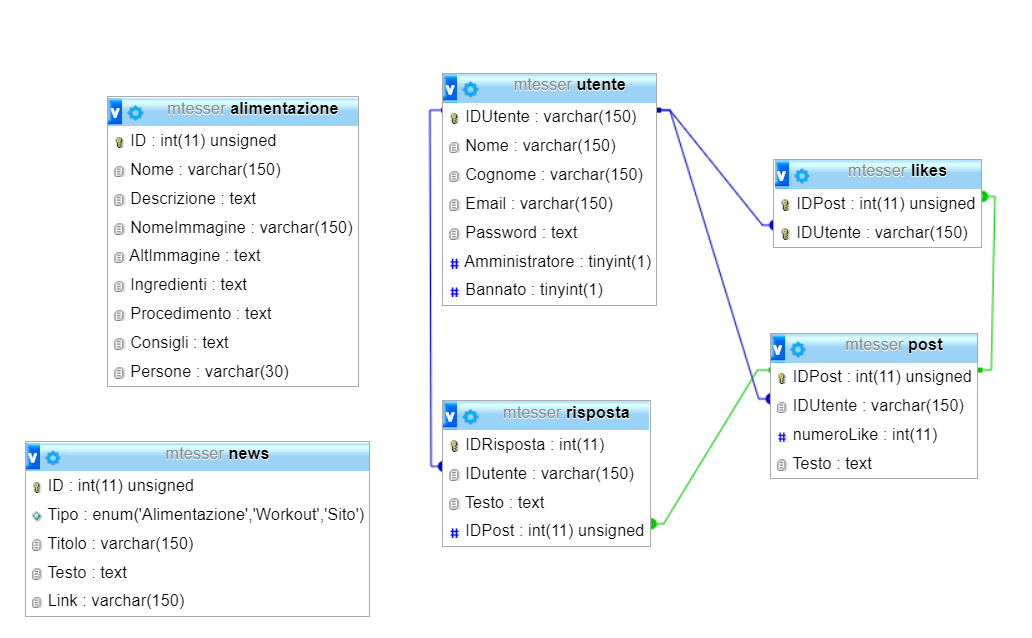
\includegraphics[width=18cm]{img/database.png}
\end{figure}
\newpage
Al fine di evitare problematiche causate dall'eliminazione dei post, quando uno di questi viene cancellato, vengono rimosse anche tutte le risposte e tutti i like. Allo stesso modo vengono eliminati anche tutti i post, 
tutti i like e tutte le risposte quando un utente viene eliminato.

\subsubsection{PHP}\label{subs:php}

Tutte le pagine del sito sono costruite dinamicamente, nella maggior parte dei casi utilizzando solamente il linguaggio PHP.\\
Ogni pagina ha un template, riconoscibile tra i file .xhtml in quanto contiene la parola \textit{base} nel nome. Ci sono 4 template nel progetto:

\begin{itemize}
    
	\item adminBase.xhtml
    \item profileBase.xhtml
	\item forumBase.xhtml
	\item base.xhtml
	
\end{itemize}

La differenza tra le varie pagine che ci ha portati a definire 4 template sono gli script Javascript che dovevano essere inclusi soltanto in alcune pagine. Queste pagine contengono la struttura base dei div, 
i quali fungono da contenitori per tutti gli elementi del sito, e che vengono costruiti dinamicamente. Tramite alcuni tag vuoti non validi riusciamo infatti a sostituire i contenuti della pagina molto velocemente tramite i parametri \textit{get}.\\

Il cuore di questo sistema sono le due classi PHP \textit{Renderer} e \textit{Parser}, che permettono di creare i contenuti delle varie pagine in base al parametro \textit{get 'r'} e ad una serie di convenzioni utilizzate per i tag vuoti. La classe Parser, infatti,
tiene in un campo privato tutte le possibili route indicate nel file index.php, una funzione e un array di variabili per ogni route. Nel file index.php alla fine viene chiamata la funzione \textit{parse}, che, se il parametro \textit{get 'r'} esiste ed è presente nel campo apposito 
del parser, renderizza il file corrispondente (tramite la classe Renderer, spiegata nel paragrafo successivo) e chiama una funzione passata durante il setup fatto in index.php. Questo permette di creare dinamicamente i contenuti utilizzando i file .xhtml.
La classe Renderer si occupa di renderizzare i file in base ai diversi tipi di placeholder, ovvero i tag vuoti, e i vari simboli speciali tramite delle funzioni di utility. 
I vari tipi di placeholder sono 4:

\begin{itemize}
    
	\item includePlaceholder
    \item blockPlaceholder
	\item ifPlaceholder
	\item variablePlaceholder
	
\end{itemize}

Ognuno di questi placeholder ha un preciso significato, riportato di seguito:

\begin{itemize}
    
	\item includePlaceholder: questo placeholder, obbligatorio, identifica una base alla pagina corrente. Si trova all'inizio della pagina e ha la forma <includeBasePlaceholder />. Il Renderer, quando trova un tag in questa forma, tramite un'espressione regolare prende il file con il nome corrispondente alla sottostringa compresa tra include e Placeholder e ne inserisce i contenuti nella pagina;
	
    \item blockPlaceholder: questo placeholder ha la forma <blockSetBlocknamePlaceholder /> e si trova in tutte le pagine. Questo placeholder indica che in quel particolare punto della pagina va inserito un blocco di codice html. Il blocco è identificato dal 
	nome, ovvero la sottostringa compresa tra Set e Placeholder. L'identificativo è infatti usato nella sostituzione del tag vuoto, in quanto il tag <blockSetBlocknamePlaceholder /> viene sostituito da tutto ciò che è compreso tra i tag <blockDefBlocknamePlaceholder /> 
	e <blockEndPlaceholder />, rimuovendo dopo la sostituzione i tag non validi e il contenuto del blocco per non avere un pezzo di codice html duplicato. I tag blockDef e blockEnd devono tuttavia essere nello stesso codice 
	sorgente in cui si trova il tag BlockSet;
	
	\item ifPlaceholder: questi placeholder hanno la forma <ifConditionPlaceholder />. Questo tipo di blocchi viene usato quando un segmento di codice deve essere renderizzato in base ad una condizione. Infatti il codice compreso tra il tag <ifConditionPlaceholder /> 
	e il tag <endIfPlaceholder /> viene inserito nel codice effettivo solamente a patto che si verifichi una certa condizione. La condizione è data dalla sottostringa compresa tra if e Placeholder. Il Renderer infatti cerca una variabile che deve essere passata al Renderer stesso e che deve essere di tipo booleano. Se la condizione è vera viene renderizzato il blocco, altrimenti no;
	
	\item variablePlaceholder: questi placeholder hanno la forma <variablePlaceholder />. Questo tipo di blocchi sono presenti in grande quantità per parametrizzare alcune parti della pagina, come per esempio il titolo delle diverse pagine. Le variabili vengono 
	passate al Renderer dal Parser, e al Parser dall'utente dal file index.php.
	
\end{itemize}

Esistono inoltre tre funzioni, messe a disposizione da Renderer, che permettono di avere un output finale valido e pulito.\\ La prima si chiama replaceEnglish ed è pensata per automatizzare l'inserimento di elementi inline, come lo span, per le parole in lingua
inglese. Questo metodo infatti ricerca tutti i segmenti di codice html compresi tra 2 simboli \% (come per esempio \%\%english word\%\%)e lo inserisce all'interno di uno span con attributi \textit{xml:lang="en"} e \textit{lang="en"}.\\ La seconda funzione permette
di rimuovere tutti i commenti dal codice HTML per rendere la pagina più leggera e avere un miglior posizionamento nei motori di ricerca. Questo è particolarmente utile nella pagina split.xhtml, in cui ci sono 4 includePlaceholder che vengono sostituiti con il 
contenuto specifico di tutte le possibili split. Questo contenuto viene poi sostituito tramite degli ifPlaceholder e infine viene rimosso il commento contenente il codice HTML di tutte le pagine.\\ La terza funzione elimina tutti i tag non validi che contengono 
il termine Placeholder, in quanto è nostro interesse far si che la pagina sia valida anche nel caso in cui qualcuno di questi tag non sia sostituito per errore.\\
I contenuti dinamici vengono gestiti tramite una classe DBaccess che permette di accedere al database e di eseguire delle query tramite la chiamata dei metodi della classe stessa, ognuno dei quali esegue una o più query al database con lo scopo di modificare 
dinamicamente i contenuti del sito sia nella creazione delle pagine che, per esempio, nelle azioni di modifica del sito che possono essere performate da un utente o da un amministratore.\\
Il file helper.php contiene invece una serie di funzioni che permettono di pulire l'input nel lato backend in modo da avere un livello di sicurezza superiore nel caso in cui un utente riesca ad aggirare i controlli di javascript.\\
Il file contentCreator.php infine contiene una serie di funzioni che creano i contenuti di alcune delle pagine utilizzando la funzione renderFile di Renderer e seguendo lo stesso principio descritto precedentemente.\\

Ci sono inoltre molti file .php nella cartella api che vengono sfruttati per il login/signup o per le chiamate asincrone di javascript (come spiegato in \S\ref{subs:js}).



\subsubsection{Javascript}\label{subs:js}

Il linguaggio javascript è stato utilizzato per il comportamento dinamico lato client delle pagine. In particolare è stato utilizzato per: 

\begin{itemize}
    
	\item Gestire il menù in modalità mobile;
    \item Controllare l'input;
	\item Popolare la pagina del forum con gli elementi che la caratterizzano nella sezione dei commenti;
	\item Popolare con i dati dell'utente la pagina del profilo;
	\item Popolare con i dati necessari la pagina del pannello admin;
	\item Gestire le modifiche o gli inserimenti fatti nella pagina profilo o nel pannello admin.
\end{itemize}

Nonostante ci sia la possibilità che un utente del sito abbia disattivato javascript, la possibilità che questa condizione si verifichi è estremamente bassa, perciò è stato deciso di gestire con questo linguaggio alcune delle pagine. 
Sappiamo inoltre che i contenuti generati con javascript non sono indicizzati dal motore di ricerca, perciò è stato utilizzato solamente per i contenuti che non devono essere necessariamente indicizzati. Di seguito i dettagli.

\paragraph{Menu mobile} % se il js è disattivato il menù si vede lo stesso in mobile? EDIT: no

Il menu mobile è stato realizzato con il linguaggio CSS. Lo script si occupa solamente di applicare o togliere alcune classi dal menu stesso in modo che sia sempre visibile in modalità desktop, e che diventi visibile o nascosto in base al click su un'immagine 
presente nel breadcrumb.

\paragraph{Controllo dell'input}

Lo script di autenticazione è molto semplice e controlla solamente che i campi non siano vuoti. La maggior parte dei controlli è infatti eseguita usando il linguaggio php nel backend. Nel caso in cui il controllo effettuato rilevi un errore di input da parte dell'utente, viene visualizzato un messaggio che spiega qual è stato l'errore. 

\paragraph{Script della pagina profilo}

Lo script della pagina profilo si occupa solamente di popolare i diversi campi input della pagina e di richiamare il php in caso di modifiche. I campi disponibili che possono essere cambiati sono: il nome, il cognome, l'email e la password. Il campo password è volutamente non compilato a causa 
del fatto che nel database è memorizzato l'hash della password. Questo script fa uso della funzione asincrona built-in di javascript, fetch, che permette di far uso di codice del backend (in questo caso con il linguaggio php) per modificare il 
front end. Tutti i file php utilizzati da questa pagina sono raccolti nella cartella api.

\paragraph{Script del pannello admin}

Lo script del pannello admin si occupa, similmente al caso della pagina del profilo, solamente di popolare i diversi campi della pagina e di richiamare il php in caso di modifiche o nel caso di nuovi inserimenti di news o ricette. 
Questo script, come il precedente, fa uso della funzione built-in di javascript fetch. 
Tutti i file php utilizzati da questa pagina sono raccolti nella cartella api.

\paragraph{Script del forum}

Lo script del forum genera la maggior parte della pagina, avvalendosi, come nei casi precedenti, di diverse funzioni fetch per prendere dal database tutti i post, le risposte e i like e costruire dinamicamente l'intera pagina, utilizzando 
\textit{document.createElement} per creare gli elementi della pagina stessa e nidificandoli uno dentro l'altro con delle funzioni anonime e ritornando gli elementi creati. 




